\chapter{Background}\label{chap:background}

\todo{remove deepTools entirely}

\todo{Add Glossary?}

\todo{use more formal language}

\todo{write poolmanagers for printing}



Chromatin usually describes different levels of how DNA organizes itself. The
well-known double-helix is only the lowest of several structural layers.
Looking at it from the outside (highest structural layer), DNA looks similar to
a big ball of wool. With the help of chromosome conformation technologies
spatial proximity can be visualized


\section{Chromosome Conformation Technologies}\label{sec:cct}


\begin{figure}[t]
\begin{centering}
    {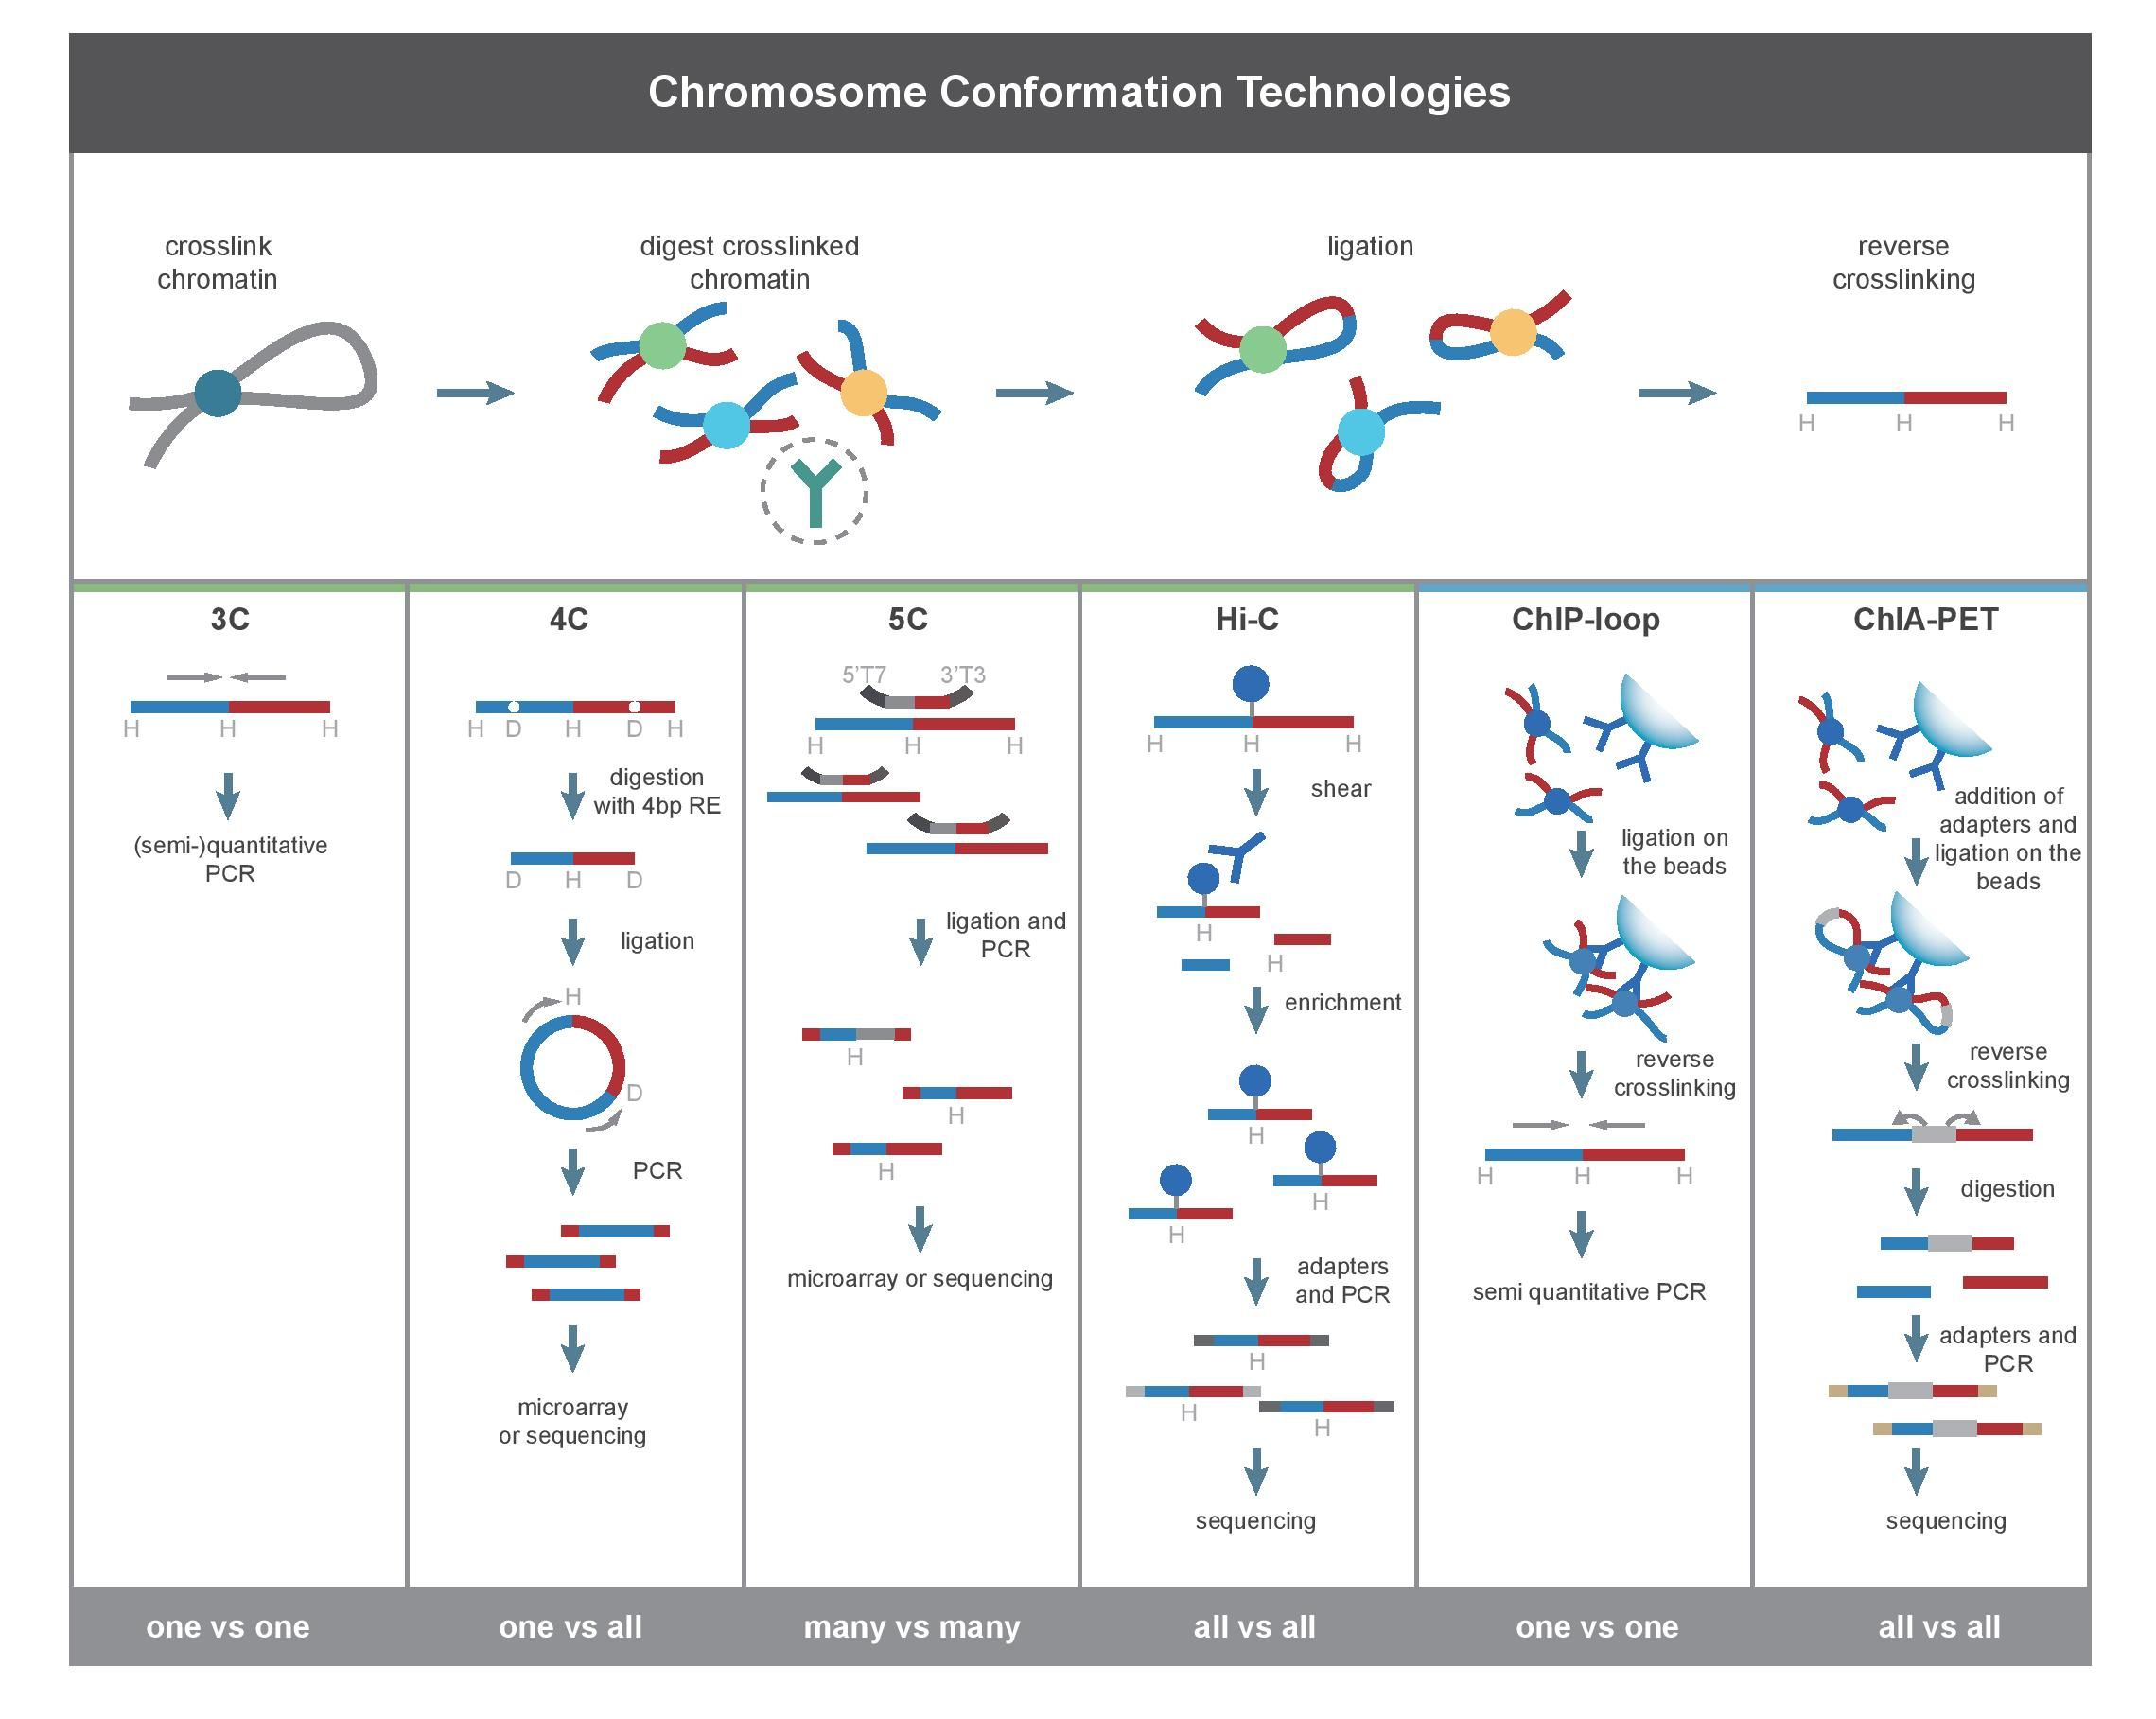
\includegraphics[scale=0.75]{figures/background/Chromosome_conformation_techniques.jpg}}
    \caption[Comparison between 3-C and its derived methods]
    {\textbf{Comparison between 3-C and its derived methods.}
    Clearly seen can be why 3-C, 4-C, 5-C and Hi-C are commonly referred to as
    3-C-based techniques.
    % ChIP-loop and ChIA-PET have these steps in a modified
    % version as well.
    \\ \\ Image from \cite{Li2014}.}
    \label{fig:comparison3C}\label{fig:cct}
\end{centering}
\end{figure}





\subsection{Common steps}\label{sec:common}

As can be seen in \figref{fig:cct}, The first steps, crosslinking, digestion,
ligation and the reversal of crosslinking, are the same for all 3-C-based methods.

\subsubsection{Cross-linking DNA}\label{sec:crosslinking}

The first step is to cross-link DNA strands that are close to each other
spatially (see \figref{fig:cct} or \figref{fig:HiC} for reference). This is done by adding
formaldehyde, which connects (links) sufficiently close strands together.

A chromatin cross-link is two entirely different parts of the genome held
together by a chemical bond with formaldehyde. This process cannot be
specifically controlled, so only `regions near each other' are connected, but
not necessarily all regions that are known to be spatially close.

\subsubsection{Digestion}\label{sec:digestion}

The next step is cutting the DNA, currently more similar to a ball of wool,
apart in intervals. For this, restriction-enzymes are used (specifically
restriction endonuclease). Commonly used enzymes for this are DpnII or HindIII,
cutting the genome every 4000 base-pairs \cite{liebermann2009comprehensive}.
This will result in a lot of cross-linked fragments, as well as
not-cross-linked ones.

\subsubsection{Ligation}\label{sec:ligation}

After reducing the concentration of fragments, DNA ligase is added, to ligate
(weld together) dangling fragment ends. For this a reduction in concentration
is done since mostly fragments close together are ligated, it is intend to
ligate fragments linked together by formaldehyde.

In HiC, Biotin is added in this step to mark ligated fragments. This allows
filtering out most fragments that have not been ligated in a later step.


\subsubsection{Reverse Cross-links}\label{sec:revcrosslink}

% Source: http://www.protocol-online.org/biology-forums/posts/10475.html
Adding a high concentration of salt for some time will reverse the
cross-linking through formaldehyde, leaving us with our two originally
spatially close fragments ligated and with a biotin-marker.


Note that at this point, the fragments are too long to sequence them.
They are ligated fragments of around 8000 base-pairs, but most current
sequencing methods can only deal with sequence lengths of a few hundred
base-pairs at most.




\subsection{3-C}\label{sec:3C} 

In 2002 Dekker et al. \cite{dekker2002capturing} developed a method test for interactions
between a single pair of genomic loci. Candidates for promoter-enhancer
interactions can be tested using this method.
After the reversal of cross-links (\secref{sec:revcrosslink}), the fragments
\extend{what is (semi-)quantitive PCR?}


\subsection{4-C}\label{sec:4C}

Chromosome conformation capture-on-chip (4C) was developed in 2006 by Simonis
et al. \cite{simonis2006nuclear}, a method to test interactions between
one genomic loci to all others. This is done by adding a second ligation-step
(see \secref{sec:ligation}, \figref{fig:cct} for reference) creating loops from
the DNA fragments and applying inverse-PCR (method to specifically amplify the
unknown parts when beginning and ending parts are known, for this the loops are
cut within the known section). Afterwards, this may get sequenced. Due to
inverse-PCR knowledge about both interacting chromosomal regions is not needed.
Results are highly reproducible for close regions \draft{find source for this}.

\extend{What is a microarray?}

% 4C (one-vs-all)
% Chromosome conformation capture-on-chip (4C) captures interactions between
% one locus and all other genomic loci. It involves a second ligation step, to
% create self-circularized DNA fragments, which are used to perform inverse
% PCR. Inverse PCR allows the known sequence to be used to amplify the unknown
% sequence ligated to it.[2][19] In contrast to 3C and 5C, the 4C technique
% does not require the prior knowledge of both interacting chromosomal regions.
% Results obtained using 4C are highly reproducible with most of the
% interactions that are detected between regions proximal to one another. On a
% single microarray, approximately a million interactions can be
% analyzed.[citation needed]



\subsection{5-C}\label{sec:5C}

Chromosome conformation capture carbon copy (5C) was developed in 2006 by
Dostie et al. \cite{dostie2006chromosome}, this method is able to test a region
for interactions with itself, such region being no bigger than a megabase. This
is done by adding universal primers to all fragments from such a region.
5-C has relatively low coverage, but is useful to analyse complex interactions
of specified loci of interest. Genome-wide interaction measuring would require
millions of 5C primers, making this method unsuitable.

% 5C (many-vs-many)
% Chromosome conformation capture carbon copy (5C) detects interactions between
% all restriction fragments within a given region, with this region's size
% typically no greater than a megabase.[2][20] This is done by ligating
% universal primers to all fragments. However, 5C has relatively low coverage.
% The 5C technique overcomes the junctional problems at the intramolecular
% ligation step and is useful for constructing complex interactions of specific
% loci of interest. This approach is unsuitable for conducting genome-wide
% complex interactions since that will require millions of 5C primers to be
% used.




\begin{figure}[t]
\begin{centering}
%    \subfloat[Diagram summarising the Hi-C experimental protocol. The red and blue rectangles represent cross-linked restriction fragments while the yellow marker shows the position of biotin incorporation.]
%    \subfloat[Generation of the Hi-C ligation junction sequence by successive digestion (with HindIII in this example), fill in and blunt-ended ligation steps. The modified restriction site sequence is not found in the original genomic sequence.]
    {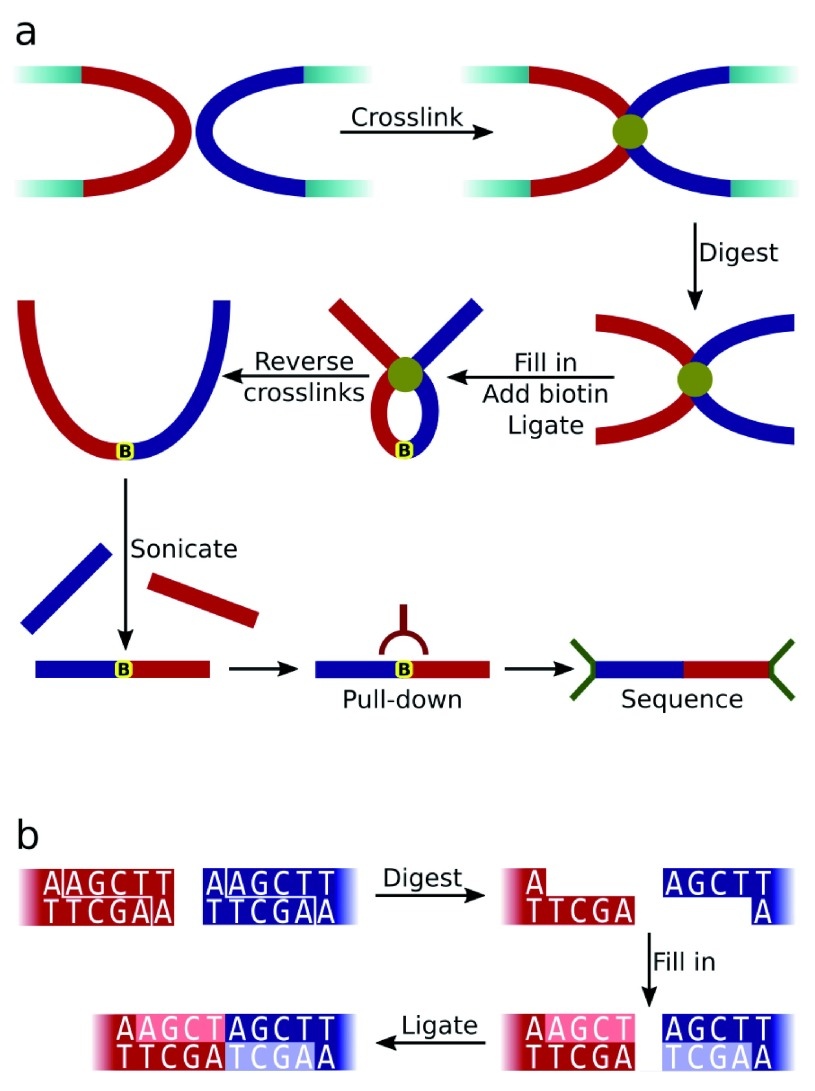
\includegraphics[scale=4]{figures/background/f1000research-4-7903-g0000.jpg}}
    \caption[Summarised Hi-C protocol]
    {\textbf{a)} Diagram summarising the Hi-C experimental protocol. The red and blue rectangles represent cross-linked restriction fragments while the yellow marker shows the position of biotin incorporation. \textbf{b)} Generation of the Hi-C ligation junction sequence by successive digestion (with HindIII in this example), fill in and blunt-ended ligation steps. The modified restriction site sequence is not found in the original genomic sequence. \\ \\ Image and description taken from \cite{wingett2015hicup}.}
    \label{fig:HiC}
    \todo{rewrite the description in my own words}

    \todo{remove the b section}
\end{centering}
\end{figure}



    % {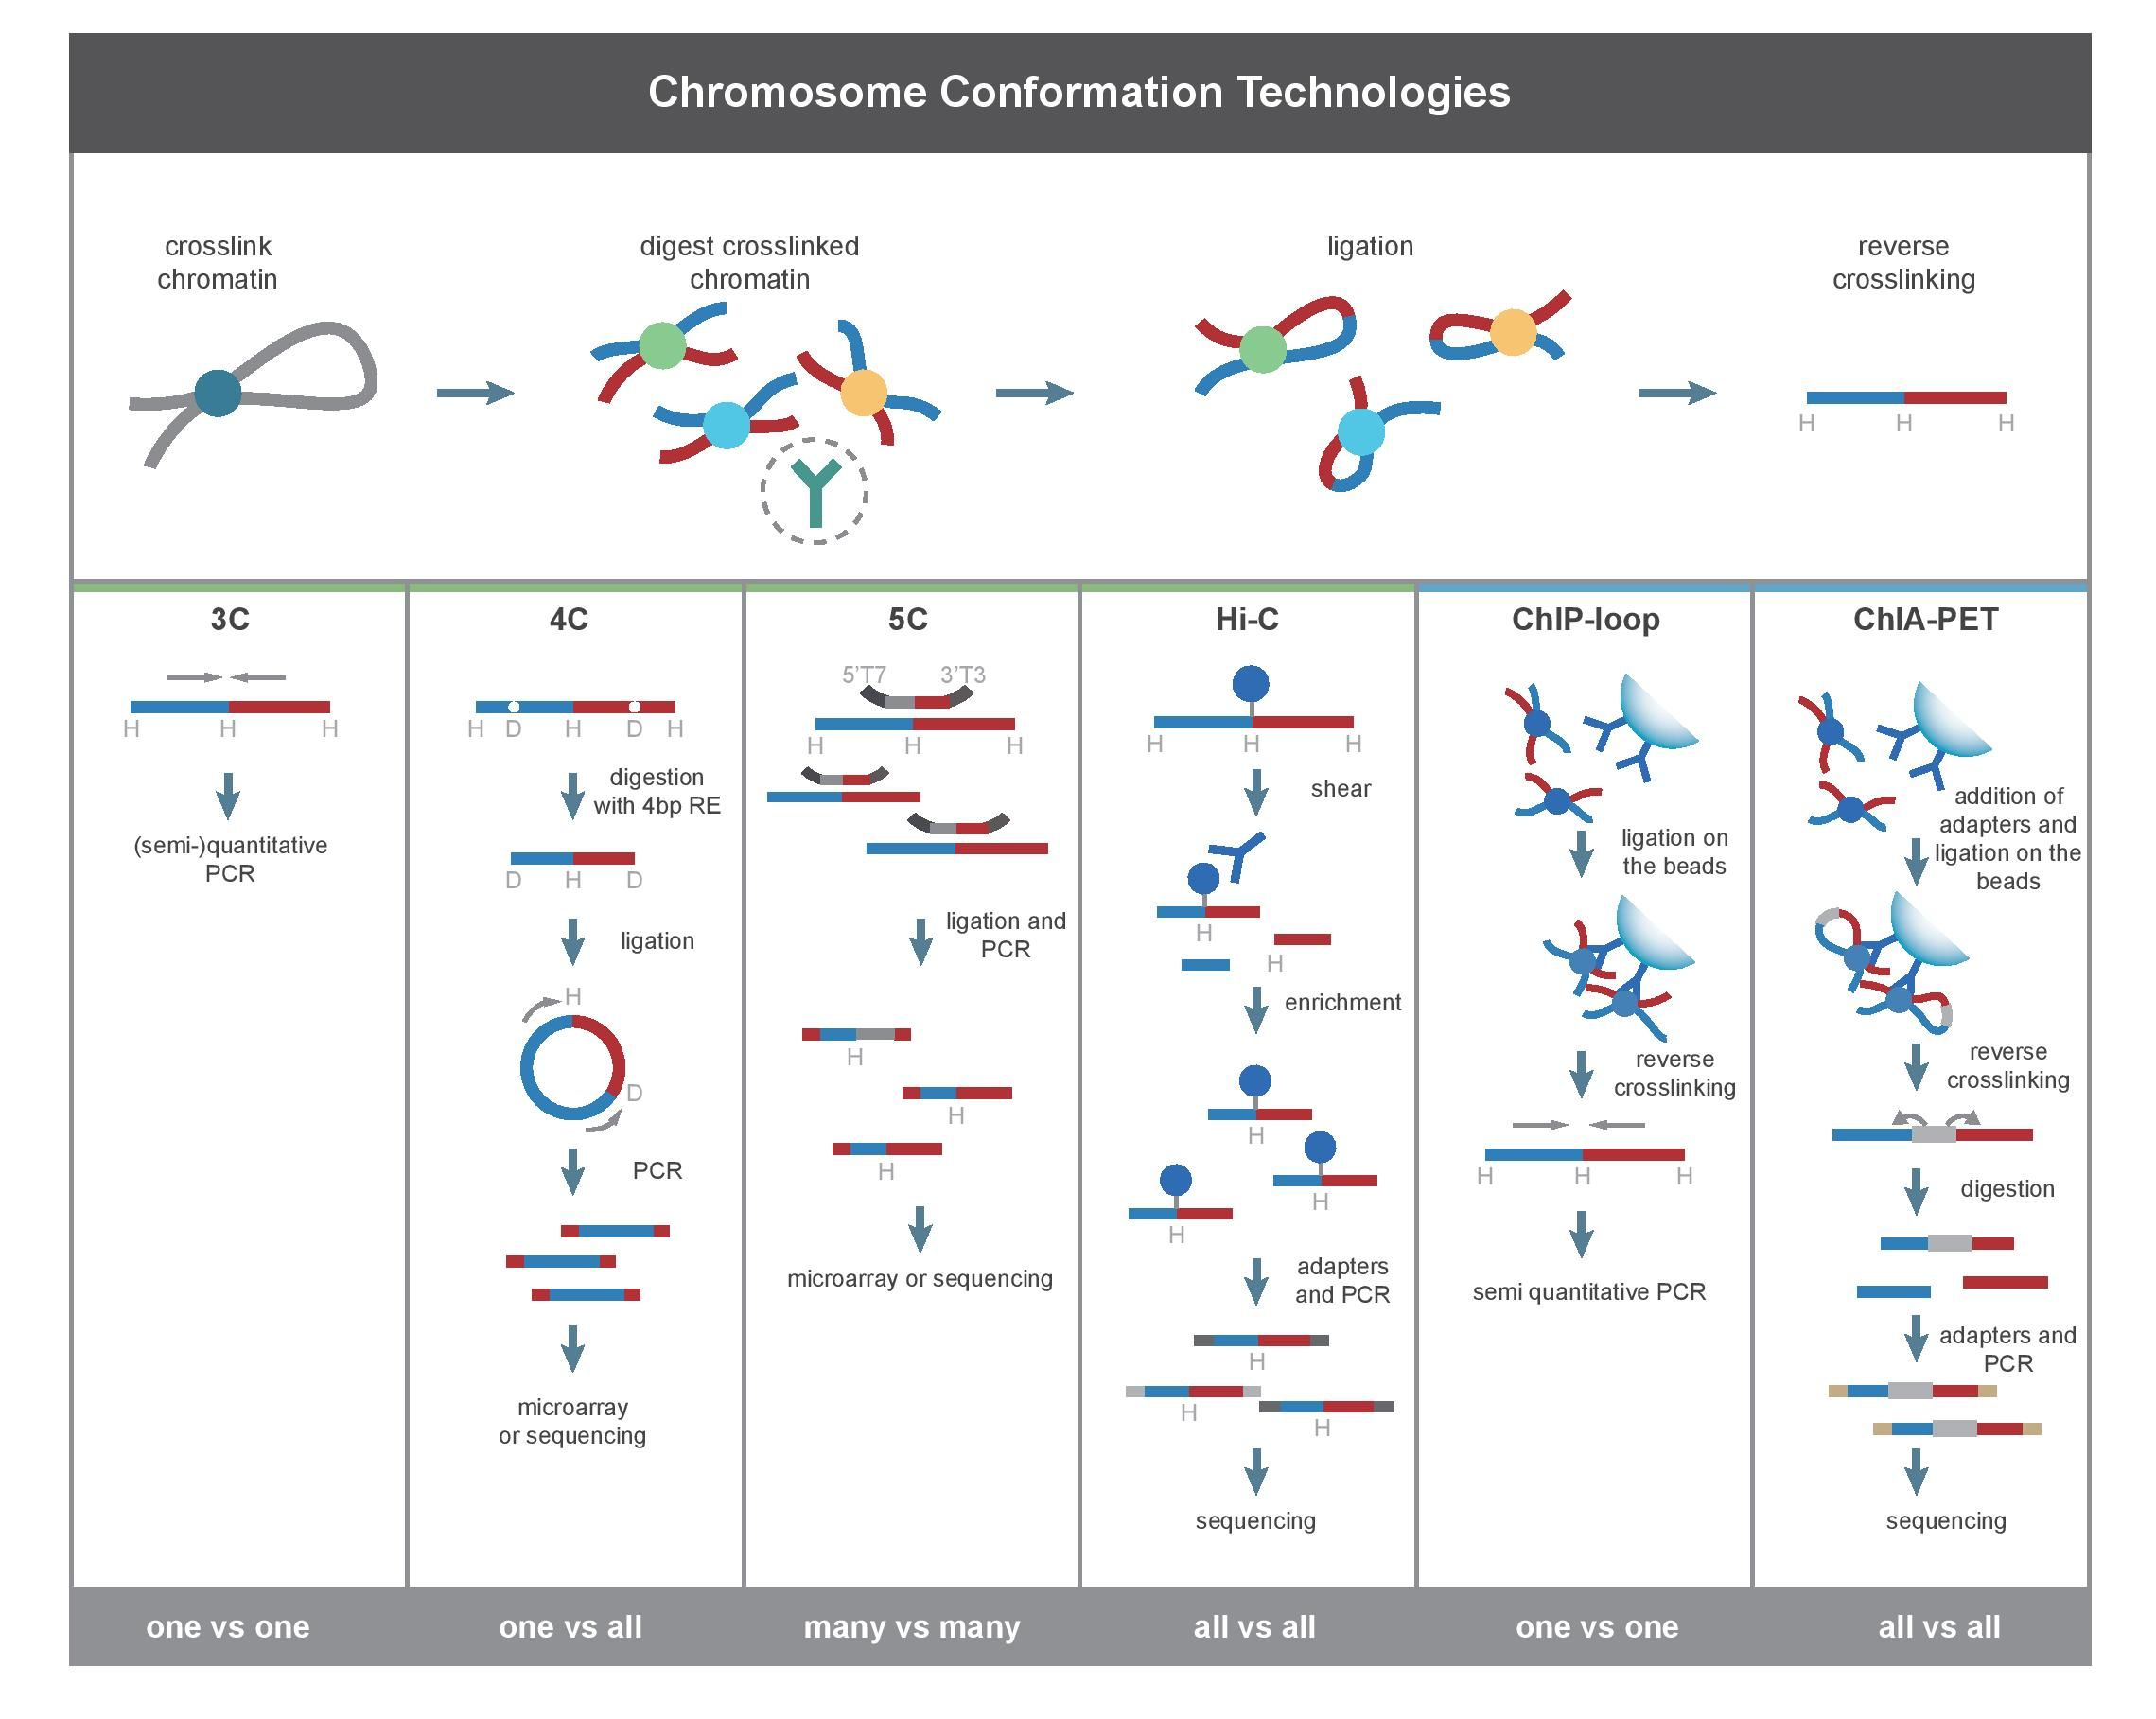
\includegraphics[scale=0.8]{figures/background/Chromosome_conformation_techniques.jpg}}
    % \caption[Comparison among 3C and its derived methods]{\textbf{Comparison among 3C and its derived methods} Source: https://en.wikipedia.org/wiki/File:Chromosome\_conformation\_techniques.jpg}


\subsection{Hi-C}\label{sec:HiC}

Hi-C (as shown by \figref{fig:hic}) was developed in 2009 by Liebermann-Aiden et al.
\cite{lieberman2009comprehensive}. After the common steps noted earlier, unique
to Hi-C is the following sequence of sonication, pulldown (filtering based on
biotin markers) and sequencing.

\subsubsection{Sonication}\label{sec:sonication}

Putting the ligated DNA-fragments under the influence of ultrasonic waves is
breaking them apart in much shorter fragments (due to long sequences not being
able to absorb frequent shocks well), shearing them apart in sequences short
enough to enable sequencing.

\subsubsection{Filtering and Removal of Biotin}\label{sec:pulldown}

`pulling-down' fragments marked with biotin leaves only those having been
marked, and thus ligated, earlier (see \secref{sec:ligation}). Subsequently the
marker is removed, as it would hinder further sequencing.

\subsubsection{Sequencing}\label{sec:sequencing}

Sequencing, short for DNA sequencing, describes processes of measuring a DNA
sequence. There are several techniques for doing this, most use PCR (Polymerase
Chain Reaction) before or while sequencing, which duplicating fragments
several times, allowing them to be sequenced more accurately.

% - putting the 3' and 5' ends there
% - usual PCR methods


% Hi-C (all-vs-all)
% Hi-C uses high-throughput sequencing to find the nucleotide sequence of
% fragments.[2][22] The original protocol used paired end sequencing, which
% retrieves a short sequence from each end of each ligated fragment. As such,
% for a given ligated fragment, the two sequences obtained should represent two
% different restriction fragments that were ligated together in the random
% ligation step. The pair of sequences are individually aligned to the genome,
% thus determining the fragments involved in that ligation event. Hence, all
% possible pairwise interactions between fragments are tested.


% Researchers attempt to study the extent of Hi-C's detection through a study
% focusing on screening primary brain tumours.[30] Prior to screening tumours,
% Hi-C was primarily focused on cell lines.[31]


\subsection{Other methods}\label{sec:other3c}

\draft{compactly explain the other methods, reference some other source}


\extend{current state}




\subsection{Overview ... ?}

\draft{stroytelling, where is all of this coming from, all these steps need to be refernced}

\todo{remove subsections and combine them}

\todo{introduce 3-C, 4-C, 5-C, then Hi-C, also add to reference}

% Gene markers tend to also have effect on their spatial neighbourhood, not only on the neighbourhood going up and down the strand of DNA.



% Chromosome conformation technologies describe several similar methods to
% compare genomic loci. They all start by:
% 
% \begin{itemize}
%     \item creating chromatin cross-links (\secref{sec:crosslinking}),
%     \item digesting the cross-linked chromatin (\secref{sec:digestion}),
%     \item ligating the ends and marking with Biotin (\secref{sec:ligation}) and
%     \item reversing the cross-link (\secref{sec:revcrosslink})
% \end{itemize}
% 
% to get a sequence with two parts, those parts have been spatially close
% to each other and were marked with Biotin during ligation.
% 
% Other chromosome conformation technologies proceed differently, Hi-C, our
% focus, continues with the following steps:
% 
% \begin{itemize}
%     \item shortening the cross-links by sonication (\secref{sec:sonication}),
%     \item filtering leaving only those with biotin (\secref{sec:pulldown}) and
%     \item sequencing (\secref{sec:sequencing}).
% \end{itemize}
% 
% The full process can be seen in \figref{fig:HiC}.

% \subsection{Cross-linking DNA}\label{sec:crosslinking}
% 
% The first step is to cross-link DNA strands that are close to each other
% spatially (see \figref{fig:HiC} for reference). This is done by adding
% formaldehyde, which bonds (links) sufficiently close strands together.
% 
% A chromatin cross-link is two entirely different parts of the genome held
% together by a chemical bond with formaldehyde. This process cannot be
% specifically controlled, so only `regions near each other' are connected, not
% necessarily two `known to be close' regions.
% 
% \subsection{Digestion}\label{sec:digestion}
% 
% The next step is cutting the ball of wool apart in intervals. For this,
% restriction-enzymes are used (specifically restriction endonuclease). Commonly
% used enzymes for this are DpnII or HindIII, cutting the genome every 4000
% base-pairs \cite{liebermann2009comprehensive}. This will result in a lot of
% cross-linked fragments, as well as not-cross-linked ones.
% 
% \subsection{Ligation}\label{sec:ligation}
% 
% After reducing the concentration of fragments, DNA ligase is added, to ligate
% (weld together) dangling fragment ends. The reduction in concentration is done
% since mostly fragments close together are ligated, and we intend to ligate
% fragments held together by formaldehyde. Also, Biotin is added to mark the
% points of ligation. This will let us filter out a lot of fragments that have
% not been ligated later on.
% 
% 
% \subsection{Reverse Cross-links}\label{sec:revcrosslink}
% 
% % Source: http://www.protocol-online.org/biology-forums/posts/10475.html
% Adding a high concentration of salt for some time will reverse the
% cross-linking through formaldehyde, leaving us with our two originally
% spatially close fragments ligated and with a biotin-marker.
% 
% Our fragments, however, are too long to sequence them effectively (remember
% that we have now ligated fragments of around 8000 base-pairs, most sequencing
% methods can only deal with sequence lengths of a few hundred base-pairs).
% 
% \subsection{Sonication}\label{sec:sonication}
% 
% The next step is to put them under influence of ultrasonic waves, breaking them
% apart in much shorter fragments (due to long sequences not being able to absorb
% frequent shocks well), short enough to actually enable sequencing.
% 
% \subsection{Filtering and Removal of Biotin}\label{sec:pulldown}
% 
% Here we `pull-down' fragments marked with biotin, filtering all the fragments
% and leaving only those having been ligated earlier (see \secref{sec:ligation}).
% Subsequently we remove the marker, since it would get in the way of sequencing.
% 
% \subsection{Sequencing}\label{sec:sequencing}
% 
% Sequencing, short for DNA sequencing, describes processes of measuring a DNA
% sequence. There are several techniques for doing this, most use PCR (Polymerase
% Chain Reaction) before or while sequencing, which duplicates the fragments
% several times, to sequence them more accurately.

% - putting the 3' and 5' ends there
% - usual PCR methods


% Open questions:
% - scaffolds?

% Chromatin is packaged into three-dimensional structures, that retain a
% relationship between genomic and physical distance. Sequences that are closer
% on the same chromosome, are also closer in physical space. Our method
% exploits this relationship between linkage and proximity to enable whole
% chromosomes scaffolding and phasing of genomes.
%
% The DNA in the sample is cross-linked in-vivo to fix DNA sequences present
% inside the same cell. Cross-linking trap sequence interactions across the
% entire genome and between different chromosomes.
%
% Cross-Linked DNA is fragmented with endonucleases. Fragmented loci are then
% biotin elated and ligated creating chimeric junctions between adjecent
% sequences. This process is called proximity ligation.
%
% The more often two sequences are joined together, the closer these two
% sequences are in genomic space.
%
% Biotinylated junctions are purified and subjected to paired-end sequencing.
% The proximity-ligation-reads are then mapped onto a draft assembly.
%
% Proximity information is used to assign context to chromosomes, and order and
% orient them along chromosome scale scaffolds.
%
% This results in fully scaffolded chromosomes of virtually any size. This
% process also detects structural variation and corrects assembly miss-joins as
% well as maps the three-dimensional conformation of chromatin within a
% population of cells.

% See \figref{fig:HiC}.


% Background:
\todo{Cite/introduce/... the given papers, and introduce the required concepts}

% Required concepts:
% \begin{itemize}
%     \item Biology:
%     \item The iterative algorithm (again ?)
%     \item analysis that can be done further
%     \item outlook. Meaning: What can be done, when having the 3C-Data?
% \end{itemize}


% \section{Further Processing}\label{sec:furtherprocessing}

% what happens after sequencing?



% \newpage
% 
% \section{deepTools}\label{sec:deeptools}
% 
% \todo{remove that entirely}
% 
% DNA sequencing is generating more data than ever before, for which deepTools,
% being a framework, has useful programs to ``process the mapped reads data for
% multiple quality checks, creating normalized coverage files in standard
% bedGraph and bigWig file
% formats''\footnote{\url{https://github.com/deeptools/deepTools}, accessed
% 2019-06-26} and more. Using these normalized, standardized files, many
% visualizations showing the actual connections or functional
% annotations, can be made.
% 
% 
\section{HiCExplorer}\label{sec:hicexplorer}

\todo{remove any mention of deepTools}
% 
HiCExplorar, being part of the deepTools-framework, is a collection of tools,
that are used to process, analyze and visualize Hi-C data. Part of this
collection are tools to convert between formats, correcting the data (which
this is work is part of), normalizing it, analysing it in various ways, and
extensively plotting it. Facilitated is, among othters ``the creation of
contact matrices, correction of contacts, topologically associating domains
(TAD) detection, A/B compartments, merging, reordering or chromosomes,
conversion from different formats including cooler and detection of long-range
contacts.''\footnotemark Those contact matrices may then be visualized, also
showing other types of data, including ``genes, compartments, ChIP-seq coverage
tracks, long range contacts and the visualization of
viewpoints''\footnotemark[\value{footnote}].

\todo{add images here about analysis}

\footnotetext{\url{https://github.com/deeptools/HiCExplorer}, accessed 2019-06-26}

% HiCExplorer facilitates the creation of contact matrices, correction of contacts, TAD detection, A/B compartments, merging, reordering or chromosomes, conversion from different formats including cooler and detection of long-range contacts. Moreover, it allows the visualization of multiple contact matrices along with other types of data like genes, compartments, ChIP-seq coverage tracks (and in general any type of genomic scores), long range contacts and the visualization of viewpoints.

% \begin{verbatim}
% hic2cool              hicCorrelate        hicPlotAverageRegions
% hicAdjustMatrix       hicDetectLoops      hicPlotDistVsCounts
% hicAggregateContacts  hicexplorer         hicPlotMatrix
% hicAverageRegions     hicFindTADs         hicPlotTADs
% hicBuildMatrix        hicInfo             hicPlotViewpoint
% hicCompareMatrices    hicMergeMatrixBins  hicQC
% hicConvertFormat      hicNormalize        hicSumMatrices
% hicCorrectMatrix      hicPCA              hicTransform
% \end{verbatim}

% analysing Hi-C data: building this interaction-matrix, correcting it,
% analysing it, compute stuff with it, ..., visualising the results.



\todo{was kann man tun mit den visualisierungen, und auf welche wege visualisiert man das etc?  Auf welchem Wege: Z.b. mit Software des HiCExplorer: hicPlotMatrix, hicPlotTADs, hicAggregate. Die Visualisierungen braucht man um komplexere Inhalte leichter (und vor allem schnell) verstaendlich zu machen. Niemand sieht z.B. in einer Matrizen sehr schnell hoehere Zahlenwerte, als Heatmap dagegen dargestellt sieht man sofort dass da ein anderes Muster in einem Bereich ist.  }


\todo{einführung in den HiCExplorer auf die ich verlinken könnte? Siehe eine der letzten Mails da hab ich ein Paper verlinkt.}




